%-----------------------------------------------
%                  Essential    
%-----------------------------------------------
\documentclass[12pt]{article}
%-----------------------------------------------
%%          %%% Hugos Template 1.7 %%%
%-----------------------------------------------
%%                  Settings
%-----------------------------------------------
%   Ändra språk och snabb compile
\usepackage[swedish]{babel}       % Språk. [swedish] eller [english].
\usepackage[]{graphicx}           % Bilder. [demo] för snabb compile!

%   Extra
%\usepackage{mhchem}              % Kemi Ekvationer.


%-----------------------------------------------
%%                  Packages
%-----------------------------------------------
\usepackage[utf8]{inputenc}  % Kodning av text.
\usepackage[]{biblatex}      % Referenser. [style=apa]
\pagenumbering{gobble}       % Stoppar sidnumrering på titelsida.

\usepackage{csquotes}        % Quotes.
\usepackage{mathtools}       % Ekvationer.
\usepackage[]{geometry}      % Sidlayout.
\usepackage{float}           % För [H].
\usepackage[T1]{fontenc}     % Bra för åäö. Kopiering.
\usepackage{microtype}       % Fixar bättre textlayout.

\usepackage[font={small,it},labelfont=bf%
,justification=centering]{caption}      % Snygg figurtext.
\usepackage{booktabs}                   % Snygga Tabeller
\setlength{\abovecaptionskip}{3pt}      % Flyttar tabelltext närmare.
\renewcommand{\arraystretch}{1.2}       % Gör tabeller större.
\setlength{\parindent}{0cm}             % Tar bort indent på ny rad.
\usepackage[none]{hyphenat}             % Slutar dela upp ord.

\bibliography{Essential/References.bib} % Mapp för Källor.
\graphicspath{{Images/}}                % Mapp för bilder.
\usepackage{pgffor}                     % Loop för bilagor.
\usepackage{pdfpages}                   % Pdfs.
\addto{\captionsswedish}{\renewcommand*%
{\contentsname}{Innehållsförteckning}}  % Ändrar namn till Innehållsförteckning

\usepackage[colorlinks]{hyperref}                  % Hyperlänkar + färg
\usepackage[nameinlink,noabbrev,swedish]{cleveref} % \cref{} & \Cref{}
\usepackage{color}                                 % Färg
\definecolor{royalblue}{rgb}{0.0, 0.14, 0.4}       % Egen färg
\hypersetup{                                       % Färg på hyperlänkar
     colorlinks  = true,
     linkcolor   = black,              % internal links
     citecolor   = royalblue,          % bibliography
     filecolor   = royalblue,          % file links
     urlcolor    = royalblue           % external links
}

\usepackage{matlab-prettifier}          % Matlab text!
\usepackage[iso,swedish]{isodate}       % Iso datum
\usepackage[per-mode=symbol]{siunitx}   % si. Skriva enheter/nummer.
\sisetup{output-decimal-marker={,},%    % si. ("{,}" till "{.}" för engelska).
range-phrase=--,range-units=single,exponent-product=\cdot}

%-----------------------------------------------
%%                New commands
%-----------------------------------------------
\newcommand{\n}{\vskip 1em}

%-----------------------------------------------
%%                Bilaga loop
%-----------------------------------------------
% Kollar om det finns .tex fil Från Bilaga_1 till Bilaga_25.
% Genererar sida om det finns.
\newcommand{\bilagaloop}{\foreach \i in {1, 2, 3, ...,25} {%
    \edef\FileName{Sections/Bilagor/Bilaga_\i}%
    \IfFileExists{\FileName.tex}{%
% Skapa .tex sida
    \newpage%
    \setcounter{page}{1}%
    \input{\FileName.tex}%
}{}}}

%%%%%%%%%%%%%%%%%%%%%%%%%%%%%%%%%%%%%%%%%%%%%%%%%%%%
%%% Creative Commons CC BY 4.0, Hugo Laestander %%%%
%%%%%%%%%%%%%%%%%%%%%%%%%%%%%%%%%%%%%%%%%%%%%%%%%%%%
%-----------------------------------------------
%%           Titelsida, ändra dessa!
%-----------------------------------------------
% Titel
\def\thetitle{En Bra Titel}
\def\theundertitle{Beskrivande Undertitel}

% Bild
\def\thefrontpage{framsida.png}

% Kurs
\def\thecourse{Kursnamn, F0000T}

% Författare
\def\theauthor{
Namn (abcdef-7@student.ltu.se) \\
Namn (abcdef-7@student.ltu.se) \\ 
Namn (abcdef-7@student.ltu.se)
}

% Handledare
\def\thesupervisor{Albert Einstein}

% Institution
\def\theinstitution{Institutionen för teknikvetenskap och matematik}

%-----------------------------------------------
%%             Titelsida layout
%-----------------------------------------------
\begin{titlepage}
	\centering
	
	% Titel
	{\Huge \textrm{\thetitle} \\}
	{\Large \textrm{\theundertitle} \\}
	\vspace{0.8cm}
	
	% Bild, ändra "height" om bilden för stor/liten
	\includegraphics[height=0.45\textwidth]{\thefrontpage}\\
	\texttt{\thecourse}\\
	\vspace{0.8cm}
	
	% Namn
	{\textbf{Författare:} \\}
	{\large \theauthor\\} % Ta bort \large ifall de behövs
	\vspace{0.8cm}
	\textbf{Handledare:}\\
	\large{\thesupervisor}  % Ta bort \large ifall de behövs
	\vfill
	
	% logga, datum
    
\includegraphics[width=0.2\textwidth]{Images/ltu_swe.jpg} \\
    \vspace{0.2cm}
    \textrm{\theinstitution} \\ \vspace{0.05cm}
	{\large \textrm{\today}\\}
\end{titlepage}

\begin{document}
\input{Essential/Style/\thetitlestyle}
\restoregeometry
\tolerance=2000
\pagenumbering{roman}
\setcounter{page}{1}

%-----------------------------------------------
%                  Sections
%-----------------------------------------------
% Skriv direkt i filerna i /Sections/...tex
% Ändra nedanstående kod vid behov.
%-----------------------------------------------
Sammanfattning av rapporten på 150-200 ord

\newpage
\tableofcontents
\hypersetup{linkcolor=royalblue}

\newpage
\section*{Beteckningar}
%
\vspace{-5mm}
\begin{table}[H]
\begin{tabular}{@{} l l l @{}}
\toprule
\textbf{Symbol} & \textbf{Benämning} & \textbf{Enhet} \\
\midrule
    $E$ & Energi & \si{J} \\
    $m$ & Massa & \si{kg} \\
    $c$ & Ljusets hastighet & \si{m/s} \\
\bottomrule
\end{tabular}
\end{table}


\newpage
\pagenumbering{arabic}

Det här är inledning.
\newpage
\section{Teori}
Det här är\footfullcite{einstein} teori \cite{einstein}.
\subsection{Underrubrik}
Hänvisning till \cref{eq:namn}
\begin{equation} \label{eq:namn}
    E=m \cdot c^2.
\end{equation}

Hänvisning till \cref{tab:namn}.
\begin{table}[H]
\centering
\caption{Tabellhuvud.}
\begin{tabular}{ l l l } \toprule
\textbf{Symbol} & \textbf{Storhet} & \textbf{Dimension} \\
\midrule
    $E$ & Energi & \si{M.L^2.T^{2}} \\
    $m$ & Massa &\si{M} \\
    $c$ & Ljusets hastighet & \si{L.T^{-1}} \\
\bottomrule 
\end{tabular} \label{tab:namn}
\end{table}

Hänvisning till \cref{fig:namn}.
\begin{figure} [H]
    \centering 
    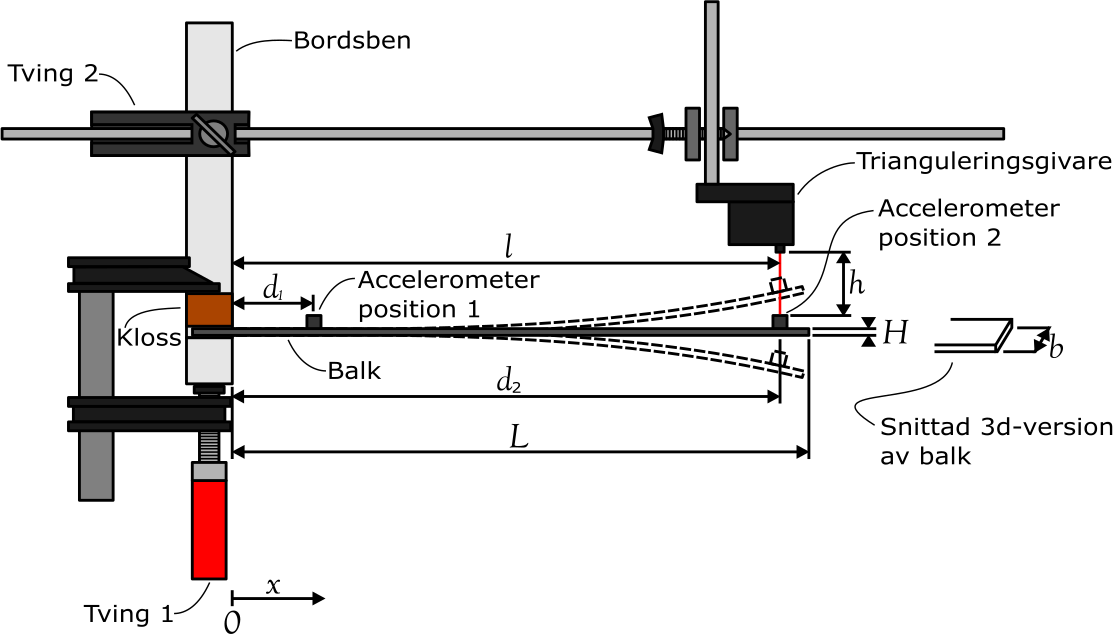
\includegraphics[width=0.5\textheight]{experiment_uppstallning.png}
    \caption{Beskrivande text.}
    \label{fig:namn}
\end{figure}
\newpage
\section{Metod} \label{s:metod}
%
Det här är metod.
\subsection{Metodbeskrivning}
\subsection{Experimentell uppställning}
Hänvisning till \cref{f:namn}.
\begin{figure} [H]
    \centering 
    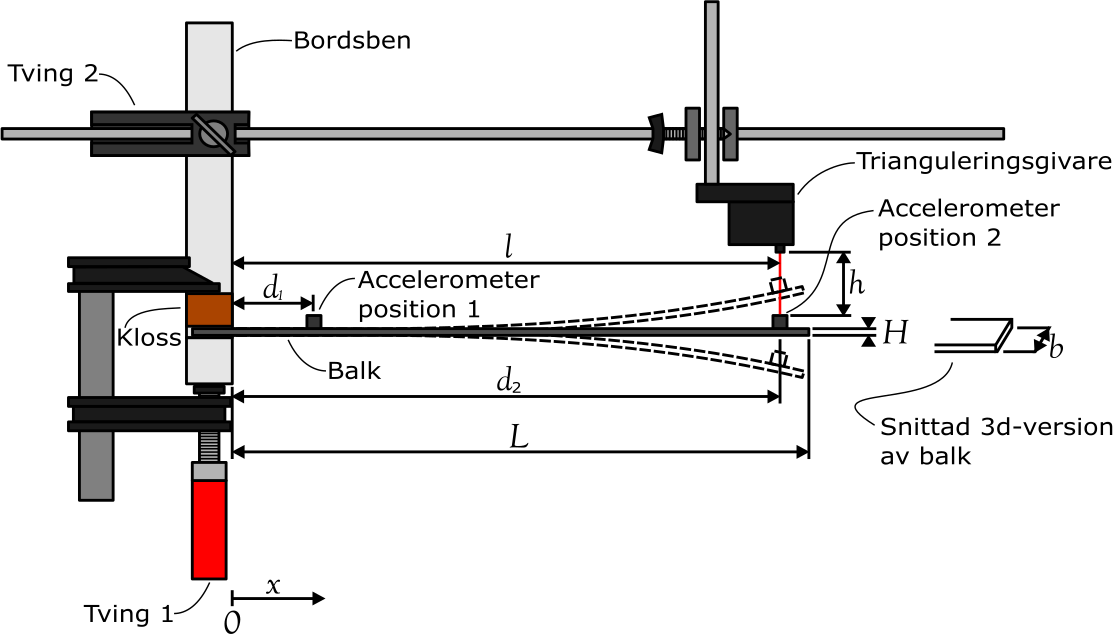
\includegraphics[width=0.5\textheight]{experiment_uppstallning.png}
    \caption{Beskrivande text.}
    \label{f:namn}
\end{figure}
\subsection{Experimentell procedur}
\newpage
Det här är resultat.
\newpage
Det här är diskussion och slutsatser.

\newpage
\printbibliography

%-----------------------------------------------
%                   Bilagor
%-----------------------------------------------
% Skapa nya filer i "Sections/Bilagor/"
% som heter Bilaga_1.tex, Bilaga_2.tex,..
% Så läggs de in automatiskt! :)
%-----------------------------------------------
\IfFileExists{Sections/Bilagor/Bilaga_1.tex}{\bilagaloop}{}
\end{document}